% paper_transparency.tex — the partial-transparency section for the eight-bot zoo (2026-10-14), PA-S', engine side.
% Replaces lines 60–166 of paper_status.tex (the thesis-era section + Discussion). Tags: [YOURS] = your prose
% kept (numbers and zoo names updated where marked), [MINE] = new text. Hinge-side results go to the appendix
% (paper_hinge_appendix.tex). Sources: app/generated/egt/runs/{body8,nonprovers+dupoc,body8+trolls,
% body8+trolls+provers,body8+natives}_sprime*; analysis in app/generated/egt/analysis/{tidy,nash_structure}.csv,
% findings.md, phase_maps.md, family_diffs.md; generators latex/scripts/gen_tau_body.py, gen_tau_ladder.py.
% Inputs: figures and tables/{tau_coop_body,tau_phase_body,tau_aggregators,tau_ladder}.tex and
% fig_tau_{summary,collapse,families}_body.pdf.

%%%%%%%%%%%%%%% Partial Transparency %%%%%%%%%%%%%%%

\section{Partial Transparency}
\label{section:Results-Transparency}
% [YOURS — "thesis" → "paper", zoo name, forward reference to the appendix]
With the base analysis done, showing that Löbian cooperation (\texttt{DupocBot}) is what selection keeps, we turn to the question this paper is about: how much transparency does that cooperation need? We run the same two analyses as in \cref{section:Results-Base}, but on the partially transparent game $G_{PD}^{\tau}(s,\alpha)$ of \cref{section:Theory-Transparency}, over a grid of transparencies $t$ and cautions $\alpha$. As in the base case, the three hinge pairs are taken at the floor side; the hinge side is re-run in \cref{apx-subsubsection:Experiments-Transparency-Hinge}.

\subsection{Setup: Zoos, Aggregators and Signals}
\label{subsection:Results-Transparency-Env}
% [MINE — replaces the thesis "Zoo" paragraph: body8 is twin-free; the ladder; the natives zoo]
\paragraph{Zoo.} The headline zoo is again the eight-bot \texttt{body}, lifted template by template. Twins matter more here than at full transparency: two programs with identical rows have behavioral distance zero, so a distance-based family can never tell them apart and its transparency has a ceiling below 1. \texttt{body} has no behavioral twins, so every family reaches $t = 1$. Two extensions serve specific comparisons. The ladder of \cref{tab:zoo-ladder} is re-run under transparency to see whether the threshold we find is a property of the roster. \texttt{body+natives} adds \texttt{MaxConfidenceBot} and \texttt{MinConfidenceBot}, so that the three aggregators over \texttt{DupocBot}'s test can be compared.

% [YOURS — unchanged]
\paragraph{Aggregators.} All lifted programs aggregate by the sum of \cref{def:Theory-Tau-Lift}: cooperate iff the cooperation mass reaches $\alpha$. The two natives keep \texttt{DupocBot}'s test, \enquote{does this hypothesis provably cooperate with me?}, and change only the vote. \texttt{MaxConfidenceBot} cooperates iff \emph{at least one} hypothesis of weight at least $\alpha$ passes the test; \texttt{MinConfidenceBot} cooperates iff \emph{every} hypothesis of weight at least $1-\alpha$ passes it, so that a single credible hypothesis that cannot be shown to cooperate vetoes. With this convention a larger $\alpha$ means more caution for all three. Because the natives are behavioral twins of \texttt{DupocBot}, the aggregator comparison is run on the $\varepsilon$-uniform family, which is identity-based and has no twin ceiling.

% [YOURS — unchanged, plus one closing sentence of mine on which family is reported where]
\paragraph{Signal families.} We use the following three parametric families, each with one internal knob ($T$ or $\varepsilon$) that is inverted numerically to reach a prescribed transparency $t$:
\begin{itemize}
    \item \textbf{Behavioral.} $s_{\mathrm{beh}}(\pi_j)(\pi_\ell) \propto \exp\bigl(-d_{\mathrm{beh}}(\pi_j,\pi_\ell)/T\bigr)$, where $d_{\mathrm{beh}}(\pi_j,\pi_\ell) := \bigl|\{\pi_m \in \mathcal{Z} : \pi_j(\pi_m) \neq \pi_\ell(\pi_m)\}\bigr|$ is the Hamming distance between the own-action rows of $\pi_j$ and $\pi_\ell$ in the outcome table.
    \item \textbf{Syntactic.} The same softmax, $s_{\mathrm{syn}}(\pi_j)(\pi_\ell) \propto \exp\bigl(-d_{\mathrm{syn}}(\pi_j,\pi_\ell)/T\bigr)$, over a normalized tree edit distance $d_{\mathrm{syn}}$ \citep{tree_signal_family} between the programs' abstract syntax trees. Its confusion structure differs from the behavioral one: for example, \texttt{DupocBot} and \texttt{CupodBot} are syntactic near-twins (one swapped action leaf) with opposite dispositions.
    \item \textbf{$\varepsilon$-uniform.} $s_{\varepsilon}(\pi_j) = (1-\varepsilon)\,\delta_{\pi_j} + \varepsilon\,\mathrm{unif}_{\mathcal{Z}}$, the structureless control: identity leaks, resemblance plays no role.
\end{itemize}
The two distance-based families are the point-mass family at $T \to 0$ and the uniform family at $T \to \infty$; the $\varepsilon$-uniform family runs from $\delta$ at $\varepsilon = 0$ to $\mathrm{unif}$ at $\varepsilon = 1$. Calibrating all three to the same $t$ is what makes them comparable: at matched $t$ every family carries the same amount of information about the opponent, so any difference between them isolates the effect of \emph{which} programs get confused with which. The headline results use the behavioral family, the syntactic family is the channel comparison, and the $\varepsilon$-uniform family is used only where a twin ceiling would confound the comparison (the aggregators).

% [YOURS — "12 to 18 distinct games" → "10 to 13"]
\paragraph{Transparency scale and grid.} For each family $s$, we set various values of $T$ and $\varepsilon$ so that their transparency $t(s)$ (\cref{subsection:Theory-Tau-Dials}) hits a target on the grid $t \in \{0, 0.2, 0.4, 0.6, 0.8, 1\}$. The caution grid we evaluate on is $\alpha \in \{0.3, 0.45, 0.62, 0.8, 1\}$. $\alpha = 0$ makes every program an unconditional cooperator and is excluded, and $\alpha = 1$ requires the whole signal to lie on cooperators. The tournament is piecewise constant in $(t,\alpha)$: grid points whose action cells coincide are the same game and share one analysis, so we report per \emph{phase region} rather than per point (36 points give 10 to 13 distinct games per sweep). One difference from the base matrix must be kept in mind: a $\tau$-program always terminates, so a proven non-termination in the base table is artificially set as a plain $D$ in the swept table.

\subsection{Results across Transparency and Caution}
\label{subsection:Results-Transparency-Analysis}
% [YOURS — numbers updated to body8: 0.31 → 0.56 and 0.25 → 0.06 at α = 0.3; 0.31 → 0.02 and 0.25 → 0.77 at α = 0.8; the α = 0.45 band now cancels exactly down to t = 0.2; the families sentence now points to the channel paragraph]
\paragraph{Cooperation rate: the sign of transparency's effect depends on caution.}
\Cref{table:tau-coop-body} gives, for the behavioral family on \texttt{body}, the fraction of ordered pairs that are $(C,C)$, exploitation, and $(D,D)$; \cref{fig:tau-summary-body} (left) plots the $(C,C)$ rate against $t$. At $\alpha = 0.3$ mutual cooperation \emph{rises} as the signal degrades, from 0.31 at $t = 1$ to 0.56 at $t = 0$, while mutual defection falls from 0.25 to 0.06: when limited information is available, trusting programs extend cooperation to programs they would defect against under full information, exploiters included. At $\alpha = 0.8$ it \emph{falls}, from 0.31 to 0.02, with mutual defection rising to 0.77: a cautious program only cooperates if most of the signal's weight lies on hypotheses it would cooperate with, and blur spreads that weight onto hypotheses it would defect against, so its threshold is no longer met.
At $\alpha = 1$ cooperation collapses at the first step below full transparency. At $\alpha = 0.45$ the two effects cancel exactly down to $t = 0.2$: the tournament does not move. The syntactic family shows the same three regimes (\cref{table:tau-coop-body} has the behavioral rates; the syntactic ones differ by at most 0.1 at any point). So the question \enquote{does transparency help cooperation?} has no unconditional answer: it depends on how cautious the programs are. Any statement about transparency has to say which $\alpha$ it holds for, which is why the rest of this section reports results over the whole $(t,\alpha)$ grid rather than along $t$ alone.

\begin{figure}[t]
  \centering
  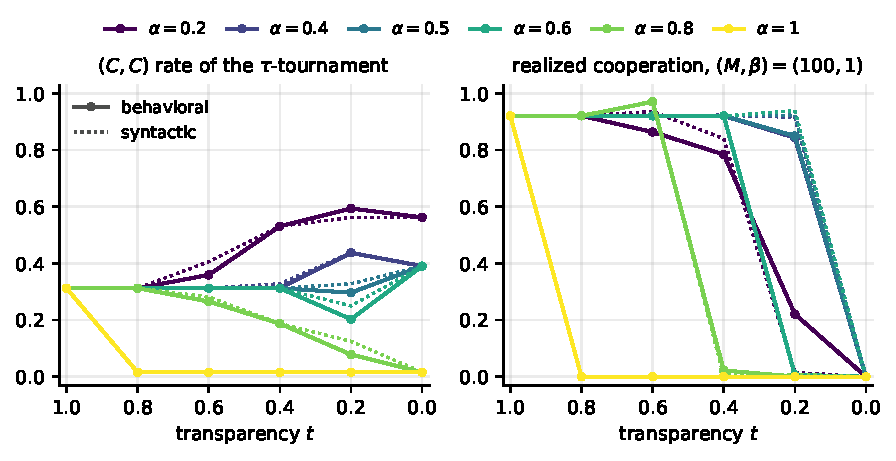
\includegraphics[width=\textwidth]{figures and tables/fig_tau_summary_body}
  % [YOURS — caption numbers updated: collapse band now between t = 0.2 and 0 for α ≤ 0.45; α = 0.62 between 0.4 and 0.2; α = 0.8 between 0.6 and 0.4]
  \caption{The two analyses over transparency, \texttt{body} zoo, behavioral family, one curve per caution $\alpha$. Left: fraction of ordered pairs that are $(C,C)$ in the $\tau$-tournament (the descriptive statistic; \cref{table:tau-coop-body}). Right: realized cooperation rate of the stationary population at $(M,\beta)=(100,1)$, i.e.\ the share of the long run spent as a monoculture whose self-play is $(C,C)$. At $t = 1$ every curve meets the base value (\cref{prop:Theory-Anchor}). Selection collapses between $t = 0.2$ and $t = 0$ for $\alpha \le 0.45$; higher caution collapses earlier ($\alpha = 0.62$ between $0.4$ and $0.2$, $\alpha = 0.8$ between $0.6$ and $0.4$, $\alpha = 1$ immediately below $t = 1$). Note the opposite behavior of the two panels at low caution: at $\alpha = 0.3$ the tournament shows \emph{more} mutual cooperation as $t$ falls, while the evolved population cooperates less.}
  \label{fig:tau-summary-body}
\end{figure}

% figures and tables/tau_coop_body.tex — tau-tournament outcome rates, body8, behavioral family, PA-S', hinge cells at the engine side (the floor value).
% GENERATED by latex/scripts/gen_tau_body.py — do not edit by hand.
% Requires: booktabs, xcolor with colortbl (\cellcolor).
\begin{table}[t]\centering\small
\caption{Outcome rates of the $\tau$-tournament on the eight-bot zoo, behavioral family, hinge cells at the engine side (the floor value): fraction of the 64 ordered pairs that are $(C,C)$ (left) and $(D,D)$ (right); the rest are exploitation pairs. Each row is one caution $\alpha$, each column one transparency $t$; the $t = 1$ column is the base matrix. Shading is proportional to the rate, green for mutual cooperation and gray for mutual defection.}
\label{table:tau-coop-body}
\begin{tabular}{@{}lcccccc@{\hspace{1.5em}}cccccc@{}}\toprule
& \multicolumn{6}{c}{$(C,C)$ rate} & \multicolumn{6}{c}{$(D,D)$ rate} \\
\cmidrule(lr){2-7}\cmidrule(lr){8-13}
$\alpha \backslash t$ & $1$ & $0.8$ & $0.6$ & $0.4$ & $0.2$ & $0$ & $1$ & $0.8$ & $0.6$ & $0.4$ & $0.2$ & $0$ \\\midrule
0.20 & \cellcolor{green!19}0.31 & \cellcolor{green!19}0.31 & \cellcolor{green!22}0.36 & \cellcolor{green!32}0.53 & \cellcolor{green!36}0.59 & \cellcolor{green!34}0.56 & \cellcolor{black!10}0.25 & \cellcolor{black!10}0.25 & \cellcolor{black!6}0.14 & \cellcolor{black!5}0.12 & \cellcolor{black!4}0.09 & \cellcolor{black!2}0.06 \\
0.40 & \cellcolor{green!19}0.31 & \cellcolor{green!19}0.31 & \cellcolor{green!19}0.31 & \cellcolor{green!19}0.31 & \cellcolor{green!26}0.44 & \cellcolor{green!23}0.39 & \cellcolor{black!10}0.25 & \cellcolor{black!10}0.25 & \cellcolor{black!10}0.25 & \cellcolor{black!10}0.25 & \cellcolor{black!5}0.12 & \cellcolor{black!6}0.14 \\
0.50 & \cellcolor{green!19}0.31 & \cellcolor{green!19}0.31 & \cellcolor{green!19}0.31 & \cellcolor{green!19}0.31 & \cellcolor{green!18}0.30 & \cellcolor{green!23}0.39 & \cellcolor{black!10}0.25 & \cellcolor{black!10}0.25 & \cellcolor{black!10}0.25 & \cellcolor{black!10}0.25 & \cellcolor{black!7}0.17 & \cellcolor{black!6}0.14 \\
0.60 & \cellcolor{green!19}0.31 & \cellcolor{green!19}0.31 & \cellcolor{green!19}0.31 & \cellcolor{green!19}0.31 & \cellcolor{green!12}0.20 & \cellcolor{green!23}0.39 & \cellcolor{black!10}0.25 & \cellcolor{black!10}0.25 & \cellcolor{black!10}0.25 & \cellcolor{black!10}0.25 & \cellcolor{black!11}0.27 & \cellcolor{black!6}0.14 \\
0.80 & \cellcolor{green!19}0.31 & \cellcolor{green!19}0.31 & \cellcolor{green!16}0.27 & \cellcolor{green!11}0.19 & \cellcolor{green!5}0.08 & \cellcolor{green!1}0.02 & \cellcolor{black!10}0.25 & \cellcolor{black!10}0.25 & \cellcolor{black!16}0.39 & \cellcolor{black!16}0.41 & \cellcolor{black!18}0.45 & \cellcolor{black!31}0.77 \\
1.00 & \cellcolor{green!19}0.31 & \cellcolor{green!1}0.02 & \cellcolor{green!1}0.02 & \cellcolor{green!1}0.02 & \cellcolor{green!1}0.02 & \cellcolor{green!1}0.02 & \cellcolor{black!10}0.25 & \cellcolor{black!31}0.77 & \cellcolor{black!31}0.77 & \cellcolor{black!31}0.77 & \cellcolor{black!31}0.77 & \cellcolor{black!31}0.77 \\\bottomrule
\end{tabular}
\end{table}


% [YOURS — rewritten numbers; one new sentence of mine (marked) on why the selected set is not the right collapse criterion]
\paragraph{Selection: a critical transparency.}
\Cref{table:tau-phase-body} shows the stochastically stable set at $(M,\beta) = (100,1)$ over the grid. On \texttt{body} under the behavioral family, \texttt{DupocBot} is uniquely stochastically stable on all of $t \in [0.4, 1]$ for every $\alpha \le 0.8$ (with \texttt{TitForTatBot} joining it at the single point $t = 0.6$, $\alpha = 0.8$), and it is still selected at $t = 0.2$ for $\alpha \in \{0.45, 0.8\}$; at $t = 0$ it either shares the set with the defectors or nothing is selected, and at $\alpha = 1$ selection dies immediately below $t = 1$.
% [MINE]
The selected set is not the right criterion for the collapse, however: \texttt{DupocBot} survives at low transparency as a \emph{defector}, since its own self-play cell turns to $(D,D)$ once the signal no longer certifies a cooperator, so the set can read \enquote{Dup} while no one cooperates. The right panel of \cref{fig:tau-summary-body} shows the quantity that matters, the cooperation rate of the evolved population.
% [YOURS — numbers updated: 0.94 → 0.92; the thresholds; "roughly 40% / 20%" → "roughly 20% / 40 to 60%"]
It stays near its full-transparency value of 0.92 and then drops to nearly zero across a band that moves with caution: between $t = 0.2$ and $t = 0$ for $\alpha \le 0.45$ (the population still cooperates at 0.78 and 0.85 at $t = 0.2$), between $0.4$ and $0.2$ for $\alpha = 0.62$, and between $0.6$ and $0.4$ for $\alpha = 0.8$; at the opaque end the surviving types, \texttt{DupocBot} among them, are all defectors. This is the first answer to our question: for cooperation to be what a population actually converges to, a trusting or moderately cautious population needs roughly 20\% transparency, and a cautious one 40 to 60\%. Full transparency is not required; near-opacity is fatal.

% figures and tables/tau_phase_body.tex — stochastically stable set at (M, β) = (100, 1), body8, both channels, PA-S', hinge cells at the engine side (the floor value).
% GENERATED by latex/scripts/gen_tau_body.py — do not edit by hand.
% Requires: booktabs, xcolor with colortbl (\cellcolor).
\begin{table}[t]\centering\small
\caption{Stochastically stable set at $(M,\beta)=(100,1)$ on the eight-bot zoo, hinge cells at the engine side (the floor value), behavioral family; where the syntactic family selects a different set the cell is shaded and reads \enquote{behavioral / syntactic}. \enquote{---} means no type reaches the stability threshold.}
\label{table:tau-phase-body}
\begin{tabular}{@{}lcccccc@{}}\toprule
$\alpha$ & $t = 1$ & $0.8$ & $0.6$ & $0.4$ & $0.2$ & $0$ \\\midrule
0.20 & \textbf{Dup} & \textbf{Dup} & \textbf{Dup} & \cellcolor{orange!25}Def+\textbf{Dup}\,/\,\textbf{Dup} & Def & Def+OB \\
0.40 & \textbf{Dup} & \textbf{Dup} & \textbf{Dup} & \textbf{Dup} & \textbf{Dup} & Def+\textbf{Dup}+OB \\
0.50 & \textbf{Dup} & \textbf{Dup} & \textbf{Dup} & \textbf{Dup} & \textbf{Dup} & Def+\textbf{Dup}+OB \\
0.60 & \textbf{Dup} & \textbf{Dup} & \textbf{Dup} & \textbf{Dup} & \cellcolor{orange!25}\textbf{Dup}+OB\,/\,\textbf{Dup} & Def+\textbf{Dup}+OB \\
0.80 & \textbf{Dup} & \textbf{Dup} & \cellcolor{orange!25}\textbf{Dup}+TFT\,/\,\textbf{Dup} & \cellcolor{orange!25}\textbf{Dup}\,/\,\textbf{Dup}+OB & \cellcolor{orange!25}\textbf{Dup}\,/\,\textbf{Dup}+OB & --- \\
1.00 & \textbf{Dup} & --- & --- & --- & --- & --- \\\bottomrule
\end{tabular}
\end{table}


% [YOURS — numbers updated; the α = 0.3 exception paragraph is gone, because on body8 the two lines drop together at every α; the ESS count is now 0 on every game]
\paragraph{The static and the dynamic collapse coincide.}
The thresholds above come from one method, the Moran process, so we check them against a second one that has nothing to do with population dynamics. For each game on the grid we ask a purely static question: does a Nash equilibrium in which both players cooperate still exist? Call the answer the \emph{static ceiling}, 1 if such an equilibrium exists and 0 if not. \Cref{fig:tau-collapse-body} draws this ceiling (dashed) together with the cooperation actually reached by the evolved population (solid), one panel per $\alpha$. In every panel the two lines drop at the same $t$: the transparency at which the cooperative equilibrium disappears is the transparency at which the population stops cooperating, for every caution on the grid. Two independent methods, one about what rational play allows and one about what selection produces, agree on the threshold. Above it, the population also nearly fills the ceiling, cooperating at 0.92 against a possible 1. Note that the static question had to be about Nash equilibria and not about evolutionarily stable strategies: none of the 22 distinct games of the two sweeps has a pure ESS, so that notion would have said nothing.

\begin{figure}[t]
  \centering
  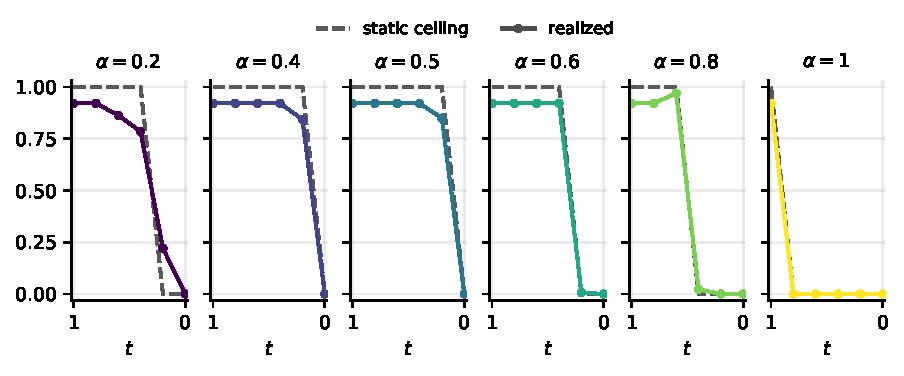
\includegraphics[width=\textwidth]{figures and tables/fig_tau_collapse_body}
  % [YOURS — "at α = 0.3 the ceiling never drops" removed; the two lines now drop together everywhere]
  \caption{Static versus dynamic collapse, \texttt{body} zoo, behavioral family, one panel per caution $\alpha$. Dashed: the static ceiling, 1 if a fully cooperative Nash equilibrium exists at that $t$ and 0 otherwise. Solid: the cooperation rate actually reached by the evolved population at $(M,\beta)=(100,1)$. The two lines drop at the same $t$ in every panel.}
  \label{fig:tau-collapse-body}
\end{figure}

% [YOURS first two sentences; the rest MINE — on body8 the channel moves who is selected but not the threshold, the opposite of the thesis finding]
\paragraph{Which programs get confused matters, but not for the threshold.}
So far the signal was behavioral: a noisy record of how the opponent plays. What if the leak is a corrupted copy of its code instead? By construction, the syntactic family carries exactly as much information as the behavioral one at the same $t$; it only differs in \emph{which} programs it mixes up. \Cref{fig:tau-families-body} shows that on this zoo the difference is real but confined to the collapse band. The two families disagree on the stochastically stable set at 5 of the 30 grid points with $\alpha > 0$, all at $t \le 0.6$, and the realized cooperation differs by more than 0.05 at four of them; but the transparency at which cooperation collapses is the same under both channels at every $\alpha$, and so is the transparency at which the cooperative equilibrium disappears. Where they differ, source blur is the \emph{more} forgiving channel: at $t = 0.2$ and $\alpha \le 0.45$ the population still cooperates at 0.92 to 0.94 under source blur against 0.78 to 0.85 under behavior blur. The pair the syntactic family confuses that the behavioral one does not, \texttt{DupocBot} and \texttt{CupodBot}, is on this zoo too (one swapped action leaf, opposite dispositions), so the mechanism is present; on an eight-bot roster its weight is simply not enough to move a threshold that sits one grid step from opacity. We read this as a property of the roster, not of the channel: a cautious population on a larger zoo may well need more transparency under source blur than under behavior blur, but we do not observe it here.

\begin{figure}[t]
  \centering
  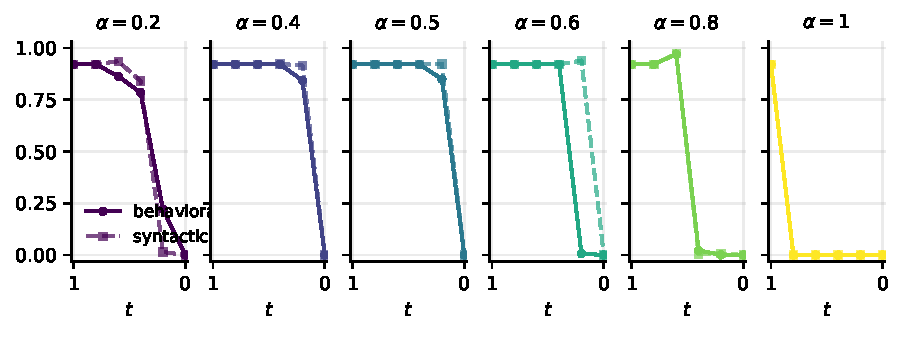
\includegraphics[width=\textwidth]{figures and tables/fig_tau_families_body}
  % [YOURS — last sentence (the EBot ESS spike) removed: there is no pure ESS on body8]
  \caption{Realized cooperation of the evolved population at $(M,\beta)=(100,1)$ under the behavioral family (solid) and the syntactic family (dashed), \texttt{body} zoo, one panel per caution $\alpha$. Both families carry the same information at equal $t$; they differ only in which programs they confuse.}
  \label{fig:tau-families-body}
\end{figure}

% [YOURS — zoo and numbers updated: Löbian class is now {Dup, Max, Min} at 93.5%; Min exits by t = 0.4 at α = 0.3 and by t = 0.2 at α = 0.45; the Max band is t = 0.2 at α = 0.62 and t = 0.4 at α = 0.8; the α = 1 row is gone from the table; one new sentence of mine on the α = 0.8, t = 0.2 cell]
\paragraph{Aggregators: pessimist $<$ expectation $<$ optimist.}
On \texttt{body+natives} under the $\varepsilon$-uniform family (\cref{table:tau-aggregators}), the Löbian class \{\texttt{DupocBot}, \texttt{Max}, \texttt{Min}\} holds 93.5\% of the long run in an even split for $t \ge 0.6$ at every $\alpha$ (down to $t \ge 0.4$ for $\alpha \in \{0.45, 0.62\}$): the aggregator is irrelevant until blur reaches the thresholds. Below that the three separate. \texttt{MinConfidenceBot}, which any credible hypothesis it cannot certify vetoes, exits first (share below 1\% by $t = 0.4$ at $\alpha = 0.3$ and by $t = 0.2$ at $\alpha = 0.45$, while \texttt{DupocBot} and \texttt{MaxConfidenceBot} split 85 to 87\% between them); in a mid-blur band \texttt{MaxConfidenceBot} alone takes 90\% ($t = 0.2$ at $\alpha = 0.62$, already $t = 0.4$ at $\alpha = 0.8$), because the sum player is fooled into cooperating with blurred exploiters while the max player, which needs one hypothesis credible on its own, is not.
% [MINE]
The band is a band of \emph{survival}, not of cooperation: at $\alpha = 0.8$ and $t = 0.2$ the sum and max players again share 88\% of the long run, but the population's cooperation rate is 0.01, since both survive as defectors.
% [YOURS]
Once identities blur, ambiguity aversion is what keeps a Löbian cooperator alive.

% figures and tables/tau_aggregators.tex — the three aggregators over DupocBot's test on body8 + natives, PA-S', engine side, epsilon family.
% GENERATED by latex/scripts/gen_tau_ladder.py — do not edit by hand.
\begin{table}[t]\centering\small
\caption{Stationary shares at $(M,\beta)=(100,1)$ on the eight-bot zoo plus the two native aggregators, $\varepsilon$-uniform family, hinge cells at the engine side. The three aggregators over \texttt{DupocBot}'s test: \enquote{sum} is the lift \texttt{DupocBot} itself, \enquote{max} is \texttt{MaxConfidenceBot}, \enquote{min} is \texttt{MinConfidenceBot}; \enquote{Löbian} is their combined share. As hypotheses the three are twins, so at $t = 1$ they are payoff-identical and the share splits evenly; they separate only once the signal blurs. Consecutive transparencies with the same shares and the same stable set are merged into one row. The last column is the stochastically stable set.}
\label{table:tau-aggregators}
\begin{tabular}{@{}llrrrrl@{}}\toprule
$\alpha$ & $t$ & sum & max & min & Löbian & stable set \\\midrule
0.20 & $\ge 0.6$ & 31\% & 31\% & 31\% & 94\% & Dup+Max+Min \\
0.20 & $0.4$ & 42\% & 42\% & 1\% & 85\% & Dup+Max \\
0.20 & $0.2$ & 1\% & 69\% & 1\% & 70\% & Def+Max \\
0.20 & $0$ & 0\% & 33\% & 0\% & 33\% & Def+Max+OB \\\midrule
0.40 & $\ge 0.4$ & 31\% & 31\% & 31\% & 94\% & Dup+Max+Min \\
0.40 & $0.2$ & 42\% & 42\% & 1\% & 85\% & Dup+Max \\
0.40 & $0$ & 0\% & 33\% & 0\% & 33\% & Def+Max+OB \\\midrule
0.50 & $\ge 0.4$ & 31\% & 31\% & 31\% & 94\% & Dup+Max+Min \\
0.50 & $0.2$ & 2\% & 85\% & 0\% & 87\% & Max \\
0.50 & $0$ & 0\% & 33\% & 0\% & 33\% & Def+Max+OB \\\midrule
0.60 & $\ge 0.4$ & 31\% & 31\% & 31\% & 94\% & Dup+Max+Min \\
0.60 & $0.2$ & 1\% & 90\% & 1\% & 92\% & Max \\
0.60 & $0$ & 25\% & 25\% & 0\% & 50\% & Def+Dup+Max+OB \\\midrule
0.80 & $\ge 0.6$ & 31\% & 31\% & 31\% & 94\% & Dup+Max+Min \\
0.80 & $0.4$ & 1\% & 90\% & 1\% & 92\% & Max \\
0.80 & $0.2$ & 44\% & 44\% & 1\% & 89\% & Dup+Max \\
0.80 & $0$ & 17\% & 17\% & 0\% & 33\% & Def+Dup+EB+Max+OB+TFT \\\bottomrule
\end{tabular}
\end{table}


% [MINE — the zoo analysis under transparency]
\paragraph{The ladder under transparency.}
Is the threshold a property of the roster? \Cref{tab:tau-ladder} repeats the behavioral sweep on the four nested zoos of \cref{tab:zoo-ladder} and reports, per caution, the critical transparency $t_c(\alpha)$: the lowest grid transparency at which the evolved population still cooperates at a rate of at least one half. On the seven-bot zoo, \texttt{body}, and \texttt{body} plus the two trolls, the thresholds agree to within one grid step: 0.2 for $\alpha \le 0.45$, 0.2 to 0.4 at $\alpha = 0.62$, 0.4 to 0.6 at $\alpha = 0.8$. The trolls change nothing, because a troll that defects against one literal program is, under any blur, a defector the Löbian test already handles. The top rung does move the threshold, downwards: with \texttt{CIMCIC} in the roster the Löbian niche is held by two programs (\texttt{CIM+Dup} is the stochastically stable set at every $t \ge 0.2$ for $\alpha \le 0.62$), the population cooperates at 0.97 to 1.00 down to $t = 0.2$, and a cautious population ($\alpha = 0.8$) makes do with 40\% transparency instead of 60\%. A second Löbian cooperator is, in effect, extra transparency: part of the signal mass a blurred \texttt{DupocBot} loses to its neighbours now lands on a program that still certifies cooperation. The threshold is therefore not a constant of the framework but of the roster, and it moves in the direction one would expect, lower with more cooperators and unchanged with more exploiters of named targets.

% figures and tables/tau_ladder.tex — the transparency ladder: critical transparency per zoo rung and caution, PA-S', engine side, behavioral family.
% GENERATED by latex/scripts/gen_tau_ladder.py — do not edit by hand.
\begin{table}[t]\centering\small
\caption{Critical transparency $t_c(\alpha)$ on the four nested zoos, behavioral family, hinge cells at the engine side: the lowest transparency on the grid $t \in \{0, 0.2, \dots, 1\}$ at which the realized cooperation of the evolved population at $(M,\beta)=(100,1)$ is still at least $\tfrac12$ (\enquote{---}: below $\tfrac12$ already at $t = 1$). The second column is the realized cooperation at full transparency.}
\label{tab:tau-ladder}
\begin{tabular}{@{}lrccccc@{}}\toprule
zoo & $N$ & coop.\ at $t{=}1$ & $\alpha = 0.3$ & $\alpha = 0.45$ & $\alpha = 0.62$ & $\alpha = 0.8$ \\\midrule
non-provers + \texttt{DupocBot} & 7 & 0.92 & $0.2$ & $0.2$ & $0.2$ & $0.4$ \\
\texttt{body} & 8 & 0.92 & $0.2$ & $0.2$ & $0.4$ & $0.6$ \\
+ trolls & 10 & 0.94 & $0.2$ & $0.2$ & $0.4$ & $0.6$ \\
+ trolls + \texttt{CIMCIC} + \texttt{DIMDID} & 12 & 0.97 & $0.2$ & $0.2$ & $0.2$ & $0.4$ \\\bottomrule
\end{tabular}
\end{table}


% [MINE — closing paragraph, replacing the Discussion section]
\paragraph{What the section says.}
On the eight-bot zoo, Löbian cooperation needs about 20\% of the information about the opponent's identity, measured as normalized mutual information, for a trusting or moderately cautious population, and 40 to 60\% for a cautious one; a unanimous one needs all of it. Above the threshold \texttt{DupocBot} is what a population converges to, exactly as at full transparency, and it cooperates at 0.92 against a static ceiling of 1; below it, cooperation stops being an equilibrium and stops being selected at the same transparency, under both channels. The selection result of \cref{section:Results-Base} therefore survives the loss of most of the information about the opponent. Critch's framework is stated at full transparency because that is where the proofs are; the population-level conclusion does not need it. Two further things the grid shows. The two analyses can point in opposite directions: at low caution the tournament's cooperation rate goes \emph{up} as the signal degrades, because trusting programs start cooperating with everyone, exploiters included, while the evolved population cooperates \emph{less}, because cooperating with an exploiter is a losing move that selection weeds out. And once identities blur, how a program aggregates the signal decides whether it survives: the pessimist exits first, the optimist last.
